% Options for packages loaded elsewhere
\PassOptionsToPackage{unicode}{hyperref}
\PassOptionsToPackage{hyphens}{url}
\documentclass[
  a4paper, twoside, 10pt, titlepage]{book}
\usepackage{xcolor}
\usepackage[a4paper, left=3.5cm, right=3cm, top=2.5cm,
bottom=3cm]{geometry}
\usepackage{amsmath,amssymb}
\setcounter{secnumdepth}{-\maxdimen} % remove section numbering
\usepackage{iftex}
\ifPDFTeX
  \usepackage[T1]{fontenc}
  \usepackage[utf8]{inputenc}
  \usepackage{textcomp} % provide euro and other symbols
\else % if luatex or xetex
  \usepackage{unicode-math} % this also loads fontspec
  \defaultfontfeatures{Scale=MatchLowercase}
  \defaultfontfeatures[\rmfamily]{Ligatures=TeX,Scale=1}
\fi
\usepackage{lmodern}
\ifPDFTeX\else
  % xetex/luatex font selection
    \setmainfont[]{Palatino}
    \setmonofont[]{Hack Nerd Font Mono Regular}
\fi
% Use upquote if available, for straight quotes in verbatim environments
\IfFileExists{upquote.sty}{\usepackage{upquote}}{}
\IfFileExists{microtype.sty}{% use microtype if available
  \usepackage[]{microtype}
  \UseMicrotypeSet[protrusion]{basicmath} % disable protrusion for tt fonts
}{}
\makeatletter
\@ifundefined{KOMAClassName}{% if non-KOMA class
  \IfFileExists{parskip.sty}{%
    \usepackage{parskip}
  }{% else
    \setlength{\parindent}{0pt}
    \setlength{\parskip}{6pt plus 2pt minus 1pt}}
}{% if KOMA class
  \KOMAoptions{parskip=half}}
\makeatother
\usepackage{longtable,booktabs,array}
\usepackage{calc} % for calculating minipage widths
% Correct order of tables after \paragraph or \subparagraph
\usepackage{etoolbox}
\makeatletter
\patchcmd\longtable{\par}{\if@noskipsec\mbox{}\fi\par}{}{}
\makeatother
% Allow footnotes in longtable head/foot
\IfFileExists{footnotehyper.sty}{\usepackage{footnotehyper}}{\usepackage{footnote}}
\makesavenoteenv{longtable}
\usepackage{graphicx}
\makeatletter
\newsavebox\pandoc@box
\newcommand*\pandocbounded[1]{% scales image to fit in text height/width
  \sbox\pandoc@box{#1}%
  \Gscale@div\@tempa{\textheight}{\dimexpr\ht\pandoc@box+\dp\pandoc@box\relax}%
  \Gscale@div\@tempb{\linewidth}{\wd\pandoc@box}%
  \ifdim\@tempb\p@<\@tempa\p@\let\@tempa\@tempb\fi% select the smaller of both
  \ifdim\@tempa\p@<\p@\scalebox{\@tempa}{\usebox\pandoc@box}%
  \else\usebox{\pandoc@box}%
  \fi%
}
% Set default figure placement to htbp
\def\fps@figure{htbp}
\makeatother
\usepackage{svg}
% definitions for citeproc citations
\NewDocumentCommand\citeproctext{}{}
\NewDocumentCommand\citeproc{mm}{%
  \begingroup\def\citeproctext{#2}\cite{#1}\endgroup}
\makeatletter
 % allow citations to break across lines
 \let\@cite@ofmt\@firstofone
 % avoid brackets around text for \cite:
 \def\@biblabel#1{}
 \def\@cite#1#2{{#1\if@tempswa , #2\fi}}
\makeatother
\newlength{\cslhangindent}
\setlength{\cslhangindent}{1.5em}
\newlength{\csllabelwidth}
\setlength{\csllabelwidth}{3em}
\newenvironment{CSLReferences}[2] % #1 hanging-indent, #2 entry-spacing
 {\begin{list}{}{%
  \setlength{\itemindent}{0pt}
  \setlength{\leftmargin}{0pt}
  \setlength{\parsep}{0pt}
  % turn on hanging indent if param 1 is 1
  \ifodd #1
   \setlength{\leftmargin}{\cslhangindent}
   \setlength{\itemindent}{-1\cslhangindent}
  \fi
  % set entry spacing
  \setlength{\itemsep}{#2\baselineskip}}}
 {\end{list}}
\usepackage{calc}
\newcommand{\CSLBlock}[1]{\hfill\break\parbox[t]{\linewidth}{\strut\ignorespaces#1\strut}}
\newcommand{\CSLLeftMargin}[1]{\parbox[t]{\csllabelwidth}{\strut#1\strut}}
\newcommand{\CSLRightInline}[1]{\parbox[t]{\linewidth - \csllabelwidth}{\strut#1\strut}}
\newcommand{\CSLIndent}[1]{\hspace{\cslhangindent}#1}
\ifLuaTeX
\usepackage[bidi=basic]{babel}
\else
\usepackage[bidi=default]{babel}
\fi
\babelprovide[main,import]{english}
\ifPDFTeX
\else
\babelfont{rm}[]{Palatino}
\fi
% get rid of language-specific shorthands (see #6817):
\let\LanguageShortHands\languageshorthands
\def\languageshorthands#1{}
\ifLuaTeX
  \usepackage[english]{selnolig} % disable illegal ligatures
\fi
\setlength{\emergencystretch}{3em} % prevent overfull lines
\providecommand{\tightlist}{%
  \setlength{\itemsep}{0pt}\setlength{\parskip}{0pt}}
\usepackage{amsmath,amssymb}
\usepackage{amsthm}
\usepackage{amsfonts}
\usepackage{float}

\usepackage{makeidx}

\usepackage[absolute]{textpos}

%Pagination stuff.
\setlength{\topmargin}{-.3 in}
\setlength{\oddsidemargin}{0in}
\setlength{\evensidemargin}{0in}
\setlength{\textheight}{9.in}
\setlength{\textwidth}{6.5in}
\pagestyle{empty}
\usepackage{bookmark}
\IfFileExists{xurl.sty}{\usepackage{xurl}}{} % add URL line breaks if available
\urlstyle{same}
\hypersetup{
  pdflang={en},
  hidelinks,
  pdfcreator={LaTeX via pandoc}}

\author{}
\date{}

\begin{document}
\frontmatter

\frontmatter

\thispagestyle{empty}

\begingroup
% \TahomaFont


\begin{textblock*}{4cm}(8.65cm,1.03cm)
	\centerline {
\includegraphics[width=3.67cm]{src/res/unito_logo.png}}
\end{textblock*}


\begin{textblock*}{21cm}(0cm,8,98cm)
	\fontsize{18}{22}\selectfont
	\centerline {\textbf{ Universit\`a degli Studi di Torino}}
\end{textblock*}
\begin{textblock*}{21cm}(0cm,9.97cm)
	\fontsize{18}{22}\selectfont
	\centerline {\textit{Corso di Laurea Magistrale in Informatica}}
\end{textblock*}


\begin{textblock*}{21cm}(0cm,13.66cm)
	\fontsize{20}{24}\selectfont
  \centerline  {\textbf{\shortstack{Concrete Numeric Representations \\ in LLM Embeddings}}}
\end{textblock*}
\begin{textblock*}{21cm}(0cm,15.46cm)
	\fontsize{18}{22}\selectfont
	\centerline{\Large {Tesi di Laurea}}
\end{textblock*}



\fontsize{14}{17}\selectfont

\begin{textblock*}{8cm}(3.04cm,18.26cm)
	\noindent
	\textbf{Relatore/Relatrice}
\end{textblock*}
\begin{textblock*}{8cm}(3.04cm,18.85cm)
	\noindent
	Prof. Di Caro Luigi
\end{textblock*}

\begin{textblock*}{8cm}(3.04cm,20.64cm)
	\noindent
	\textbf{Correlatore/Correlatrice}
\end{textblock*}
\begin{textblock*}{8cm}(3.04cm,21.23cm)
	\noindent
	Dr. Torrielli Federico
\end{textblock*}

\begin{textblock*}{8cm}(12.33cm,22.95cm)
	\noindent
	\textbf{Candidato/a}
\end{textblock*}
\begin{textblock*}{8cm}(12.33cm,23.55cm)
	\noindent	\textbf{Gentiletti Emanuele}
\end{textblock*}
\begin{textblock*}{8cm}(12.33cm,24.14cm)
	\noindent	900831
\end{textblock*}

\begin{textblock*}{21cm}(0cm,27.34cm)
	\centerline{Anno Accademico 2024/2025}
\end{textblock*}

\endgroup

\newpage
$ $

\newpage
$ $

%\mainmatter
%\TPoptions{absolute=false}
%\pagestyle{plain}
%\setcounter{page}{1}
%\newpage
%$ $

{
\setcounter{tocdepth}{2}
\tableofcontents
}
\mainmatter
\chapter{Introduction}\label{introduction}

This thesis explores LLMs from the perspective of their embeddings, in
particular their numerical ones. There are several reasons why I came to
be interested in this topic, the first and naive one being that
tokenization schemes, as naively implemented with the BPE algorithm,
would leave a lot of space for improvement in numerical tasks, and it's
interesting to explore how.

Better performance in LLMs has been sought through the lenses of scale,
and looking for emergent properties as training time and resources
increase. There are different reasons for this, one of them being The
Bitter Lesson (\citeproc{ref-bitter-lesson}{Sutton, 2019}), a heuristic
principle that states that general methods that better leverage
computation are better than methods that seek to use human
domain-specific knowledge to inform the implementation. This has been
observed, for example, in the domain of chess, where the strategies
being put forward hard-coding human domain-specific knowledge were
ultimately beaten by deep search.

After the big success story of scaling in LLMs, the main reach has been
towards increasing model size and training on bigger datasets, and in
unlocking the emergent capabilities that would come along those. While
this approach has given results, albeit with some inconsistencies hard
to reconcile from an epistemological perspective, such as the difficulty
of actually designing good benchmarks for those abilities that actually
verify they go beyond memorization (\citeproc{ref-skalse2023}{Skalse,
2023}), this road would lead to the monopolistic control of the best
version of this tool to the actors that are able to get access to the
most amount of data.

If ``Scale is all you Need'' and LLM improvement is purely a game of
resource accumulation, we would be in a situation that could exacerbate
the inequalities we're living under at the present time, leading
effectively to a crystallization of the power structures that, as of
today, have the biggest capacity for data collection. As the state of
the art gets better, the barriers of entry rise in terms of performance,
training data and hardware required to have a model that performs
competitively. As such, it is of primary importance to find strategies
to break through the massive resource requirements needed for AI
training and performance, and find alternatives that allow for a less
resource-intensive development of the field.

What is investigated here are some possible improvements that don't come
directly from training, but from a better understanding of how, through
learning, the model weights that allow LLMs to function come to be. This
comes through thought experiments about human cognition, and anomalous
cases of it (in particular, we'll take a look at Savant syndrome and
what it can tell us in the context of learning), as well as recent
research put forward about LLM capabilities in the specific field of
math.

In particular, one thing I want to propose is that the representation of
numbers can be a gateway to better understanding LLM representations in
general, as their object of representation is the same as the object
being represented (in both cases numbers), allowing to look for the
relations between the two using mathematical methods of analysis.

\chapter{Background}\label{background}

\section{The inductive bias of
Tokenization}\label{the-inductive-bias-of-tokenization}

Modern LLMs are mostly autoregressive models built on the Transformer
architecture (\citeproc{ref-vaswani2023}{Vaswani et al., 2023}).
Transformers are a deep learning architecture based on attention, a
mechanism that relates words in different positions in a sentence by
computing weighted relationships between all input tokens, allowing the
model to capture long-range dependencies and contextual relationships
that sequential models like RNNs struggle with. The first step in most
Transformer models is tokenization, which operates by converting input
text into sequences of discrete tokens that are then mapped to
high-dimensional vector representations. This initial step creates an
inductive bias that shapes how the model processes information
(\citeproc{ref-ali2024}{Ali et al., 2024};
\citeproc{ref-singh2024}{Singh \& Strouse, 2024}), with significant
implications for the application of numerical data to arithmetical
tasks.

The most used algorithm for tokenization is currently Byte-Pair Encoding
(\citeproc{ref-radford2019}{Radford et al., 2019}), which, given a fixed
vocabulary size, starts with individual characters and iteratively
merges the most frequently occurring pairs of adjacent tokens until the
vocabulary limit is reached. This process naturally creates longer
tokens for common substrings that appear frequently in the training
data. For numbers, this means that frequently occurring numerical
patterns like ``100'', ``2020'', or ``999'' might become single tokens,
while less common numbers get broken into smaller pieces. The result is
an idiosyncratic and unpredictable tokenization scheme where similar
numbers can be tokenized completely differently based purely on their
frequency in the training corpus. While GPT-2 used to have a purely BPE
tokenizer, the successive iteration of GPT and generally more recent
models either tokenize digits separately (so as
\('1234' \rightarrow [1, 2, 3, 4]\)), or tokenize clusters of 3 digits,
encompassing the integers in the range 0-999.

Most of the tokenizers right now do L2R (left-to-right) clustering
(\citeproc{ref-millidge2023}{Millidge, 2023}), meaning that a number
such as \(12345\) would be divided in two tokens, \(123\) and \(45\). It
has been shown (\citeproc{ref-singh2024}{Singh \& Strouse, 2024}) that
this kind of clustering leads to worse arithmetic performance, as this
brings misalignment in digit positions and, as a consequence, in
positional significance.

An even more surprising development is that forcing the R2L token
clustering of numbers in models already trained with L2R clustering
through the use of commas in the input (ex. \(12,345\)) leads to big
improvements in arithmetic performance
(\citeproc{ref-millidge2024}{Millidge, 2024};
\citeproc{ref-singh2024}{Singh \& Strouse, 2024}). Despite the model
learning representations adapted to work with a L2R token clustering
strategy, forcing a R2L clustering at inference time shows substantial
improvements in arithmetic tasks, which means that despite being learned
through an unfavorable tokenization approach, the numeric
representations retain the properties that allow for the performance to
improve when the digit clustering scheme is corrected.

\begin{figure}
\centering
\pandocbounded{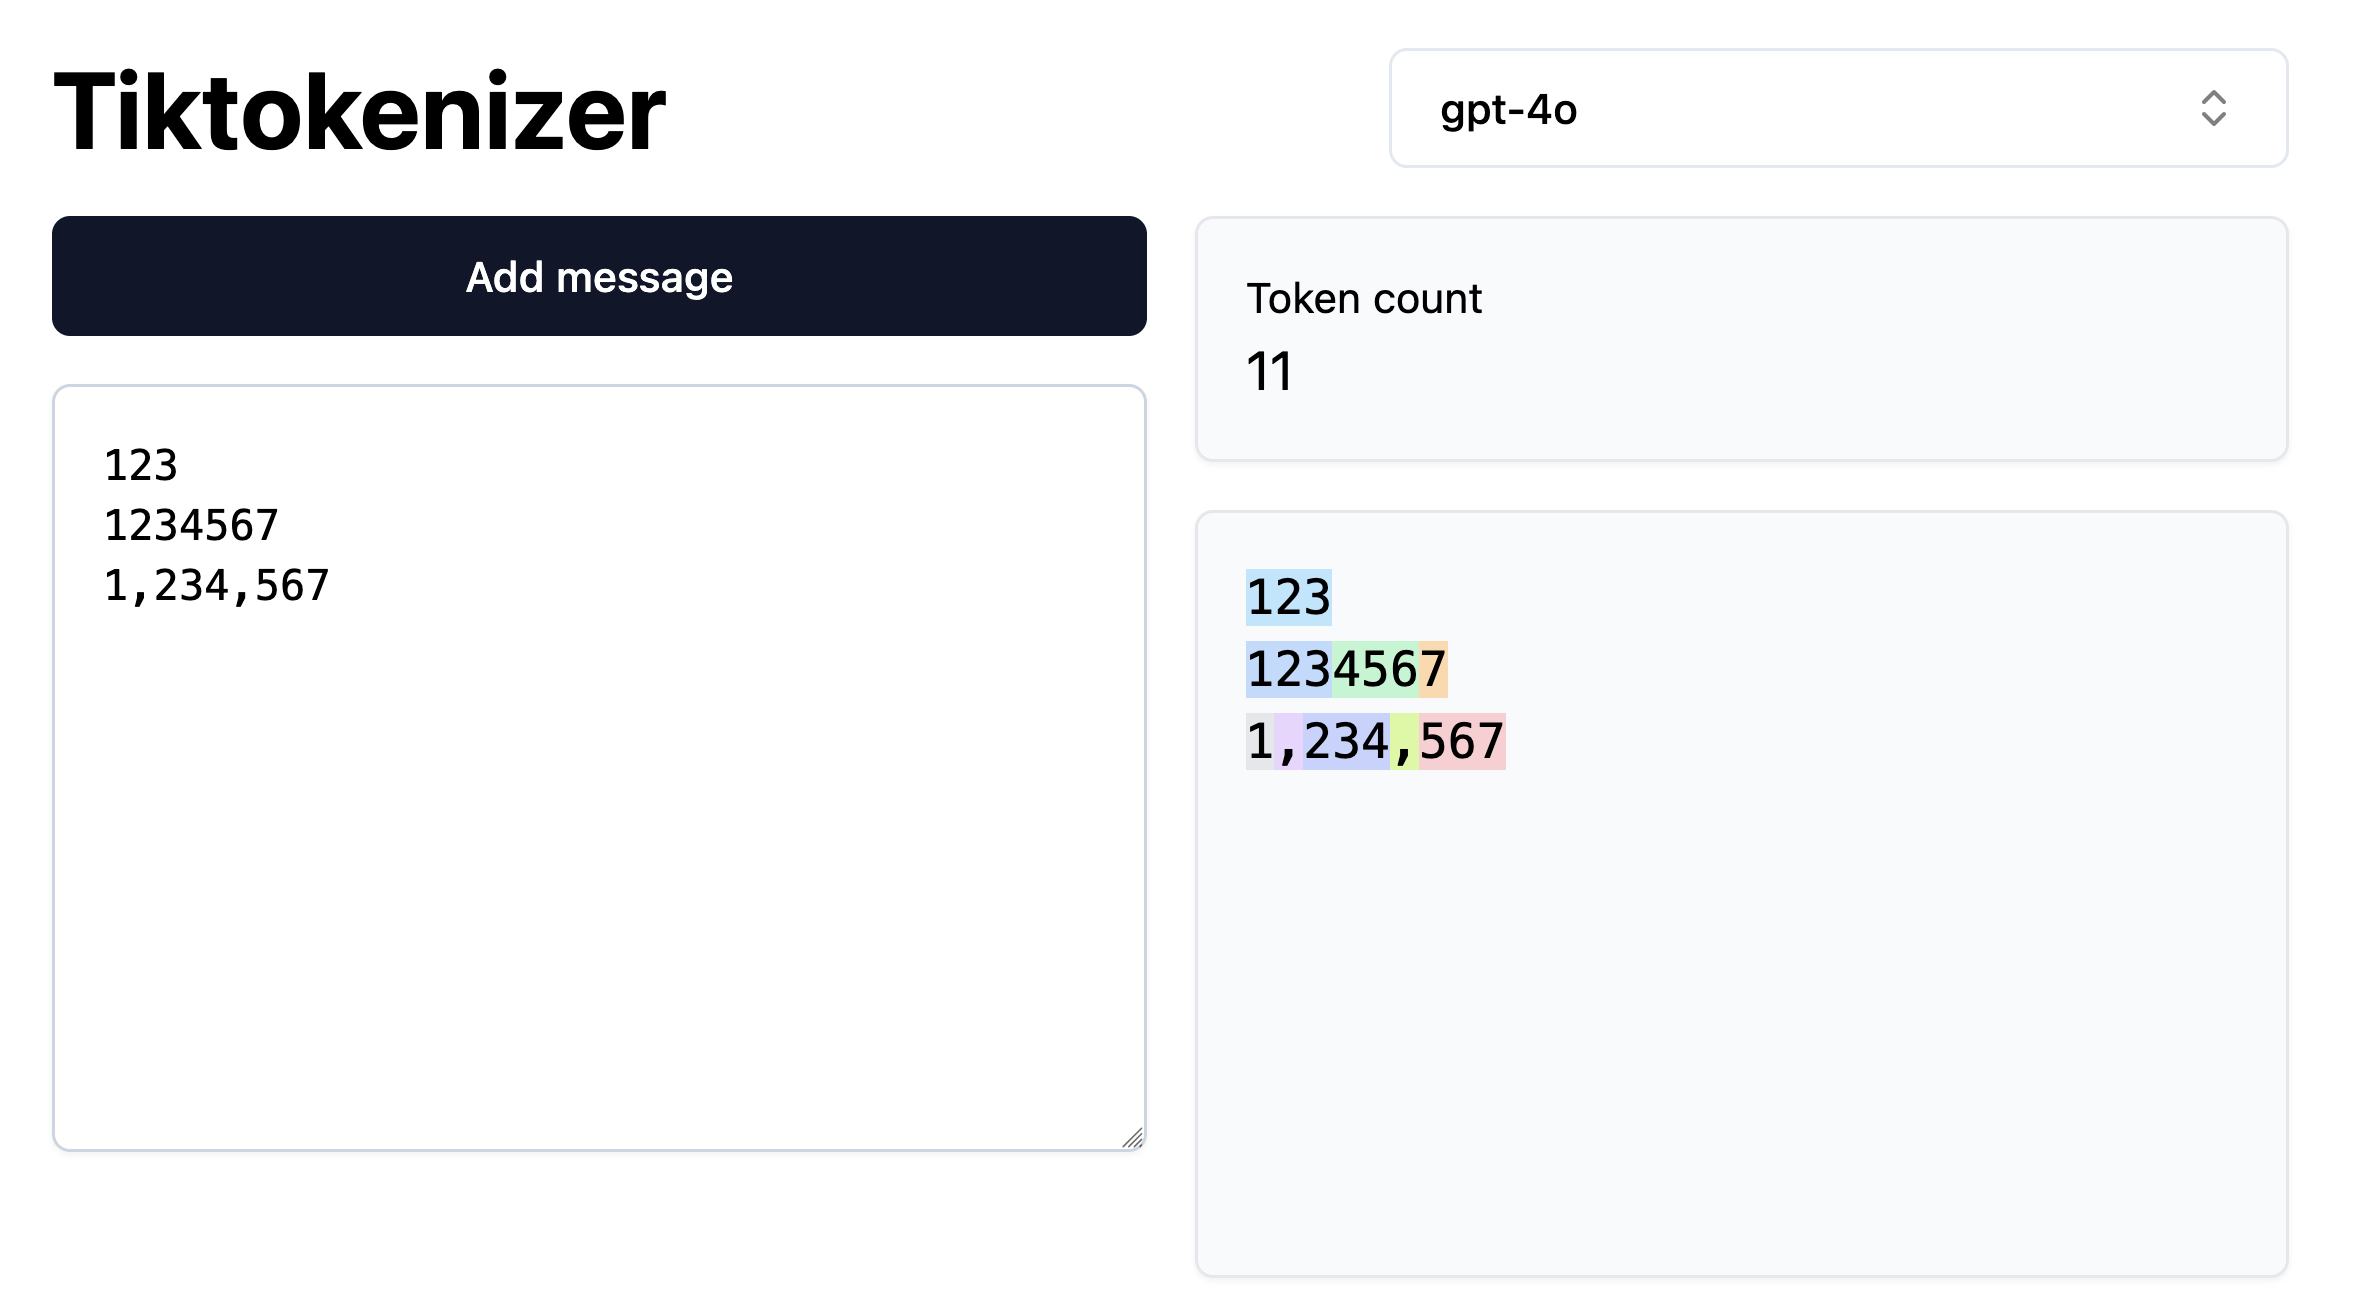
\includegraphics[keepaspectratio]{res/gpt4o-tokenization.png}}
\caption{GPT-4o tokenization of different numerical quantities,
displaying the L2R clustering and the comma trick to force R2L
clustering.}
\end{figure}

There can be different hypotheses on why this might be, for example:
arithmetic operations would still work locally in the 0-999 range, which
allows for a correct reading on them and possible generalization on a
larger scale; the forced tokenization also happens in the data, as
numbers are often separated by punctuation in clusters of 3 digits,
right to left, for legibility reasons (\citeproc{ref-singh2024}{Singh \&
Strouse, 2024}); or, as it will be explored later, an underlying
self-correcting learning structure.

At the very least, the data being biased towards a R2L representation
(in the form of using the Arabic number system and adopting legibility
rules that accommodate right to left calculations) leads to embeddings
that maintain that bias even when learned in a L2R fashion. This can be
a possible hint towards the optimality of certain representations
compared to others, given the resilience in preferring a certain
tokenization scheme over the one the model is trained on.

\begin{longtable}[]{@{}ll@{}}
\toprule\noalign{}
\textbf{Model} & \textbf{Strategy} \\
\midrule\noalign{}
\endhead
\bottomrule\noalign{}
\tabularnewline
\caption{Language models with their respective tokenization strategy for
numbers.}
\endlastfoot
LLaMA 1 \& 2 & Single digit \\
LLaMA 3 & L2R chunks of 3 digits \\
OLMo 2 & L2R chunks of 3 digits \\
GPT-2 & Pure BPE \\
GPT-3.5 / GPT-4 & L2R chunks of 3 digits \\
Claude 3 / Claude 4 & R2L chunks of 3 digits \\
\end{longtable}

\section{Strategies for mathematical improvements through
embeddings}\label{strategies-for-mathematical-improvements-through-embeddings}

Beyond better tokenization, there have been other, more comprehensive
approaches to the improvement of the representation of numeric values.
xVal is a notable one, as its approach encompasses real numbers beyond
just integers and does away with learning different representation for
each number.

The idea is maximizing the inductive bias in the representation by
having embeddings that are computed based on the number to be
represented (\citeproc{ref-golkar2023}{Golkar et al., 2023}). Numerical
values represented by a single embedding vector associated with the
\passthrough{\lstinline![NUM]!} special token.

This fits very well with the idea of reification, which will be
described later(\citeproc{ref-murray2010}{Murray, 2010}): the embedding,
beyond its qualities as representational object, becomes an entity with
features that actively aid in the calculation process.

The model uses two separate heads for number and token predictions. If
the token head predicts a \passthrough{\lstinline![NUM]!} token as the
successor, the number head gets activated and outputs a scalar. The rest
of the weights in the transformer blocks are shared, allowing the
learning of representations that are useful for both discrete text
prediction and continuous numerical prediction. This means the model
develops number-aware internal representations throughout all its
layers, not just at the output. The shared weights force the model to
learn features that work for both linguistic and mathematical reasoning
simultaneously.

The approach is shown to improve performance over a series of other
techniques, mostly using a standard notation to represent numbers
(\citeproc{ref-golkar2023}{Golkar et al., 2023}). This work has been
inspired by the xVal paper, with one of its initial goals being to find
good representations for computed numerical embeddings.

There are several different approaches to improving math performance in
LLMs that don't necessarily come directly from training, but from a
better understanding of how representations work. Other approaches
include giving models better positional information about digits within
numbers, such as Abacus Embeddings (\citeproc{ref-mcleish2024}{McLeish
et al., 2024}), which encode each digit's position relative to the start
of the number and can improve arithmetic performance substantially.

While on one hand particular modes of numerical cognition can be
explored through explicitly reifying the representation (through the
xVal approach), what the rest of the analysis hinges on is whether LLMs
develop such structures on their own, by looking at their embeddings, as
this could hypothetically inform us on how to build these structures
ourselves in a more direct way than training.

\section{Cognitive science - Savant syndrome and spatial
representations}\label{cognitive-science---savant-syndrome-and-spatial-representations}

A case study of savant patient DT (\citeproc{ref-murray2010}{Murray,
2010}) reveals a mathematical cognitive architecture with the following
characteristics:

\begin{itemize}
\tightlist
\item
  has sequence-space synesthesia with a ``mathematical landscape''
  containing numbers 0-9999
\item
  each number possesses specific colors, textures, sizes, and sometimes
  movements or sounds
\item
  prime numbers have distinctive object properties that distinguish them
  from other numbers
\item
  arithmetic calculations happen automatically
\item
  solutions appear as part of his visual landscape without conscious
  effort
\item
  fMRI studies showed that even unstructured number sequences had
  coherent visual structure for DT.
\end{itemize}

Murray argues that savants possess highly accessible concrete
representations of abstract concepts, for which she uses the term
reification - the conversion of abstract concepts into concrete, spatial
entities that can be directly ``inspected'' rather than computed.

Sequence-space synesthesia is the spontaneous visualization of numerical
sequences in organized spatial arrangements. The remarkable mathematical
abilities of savants with this condition suggest that their specialized
perceptual representations confer significant computational advantages
over normal human numerical calculation abilities.

Given that the spatial arrangement confers advantages in numerical
calculation to the subject, we can pose the question: are there specific
spatial arrangements that enable advantageous numerical calculations,
and are those present or replicable in LLMs? The spatial idea is easily
translatable from the perceptive sphere to the representational one, by
considering LLM embeddings. This also requires the assumption that
representational advantages can translate from humans to LLMs.

According to (\citeproc{ref-huh2024}{Huh et al., 2024}) AI models,
particularly deep networks, are converging. The central hypothesis is
that different models are converging toward a shared statistical model
of reality, akin to Plato's concept of an ideal reality. This
representation is termed the Platonic representation.

This convergence appears to be driven by several selective pressures:
larger models have more capacity to find optimal representations; models
trained on more diverse tasks are constrained to find solutions that
work across multiple domains; and deep networks have implicit biases
toward simpler solutions (\citeproc{ref-huh2024}{Huh et al., 2024}).

For the investigation of numerical representations, this suggests that
if there are indeed optimal geometric structures for mathematical
reasoning, different models might naturally converge toward them during
training. The shape suggested (the helix) has properties on an
information-theory basis that make its use as a learning geometry more
likely, in particular, its self-similarity can be an error-correcting
property.

\section{Dimensionality reduction and Embedding
Visualization}\label{dimensionality-reduction-and-embedding-visualization}

To visualize and analyze the high-dimensional embedding spaces that LLMs
use for numerical representations, we need techniques that make the
underlying structure evident. For this reason, we employ the following
dimensionality reduction techniques:

\begin{itemize}
\item
  \textbf{SVD (Singular Value Decomposition)} is a fundamental matrix
  factorization that decomposes any matrix \(A\) into three component
  matrices: \(A = U\Sigma V^T\), where \(U\) and \(V\) contain
  orthogonal vectors (left and right singular vectors respectively) and
  \(\Sigma\) contains the singular values on its diagonal. SVD reveals
  the underlying structure of the matrix by identifying the principal
  directions of variation and their relative importance through the
  singular values.
\item
  \textbf{PCA (Principal Component Analysis)} emerges as a specific
  application of SVD. By applying SVD to a centered data matrix (where
  each variable has been mean-centered), the right singular vectors
  \(V\) become the principal components - the directions of maximum
  variance in the data. The singular values in \(\Sigma\) are directly
  related to the eigenvalues of the covariance matrix.
\item
  \textbf{t-SNE (t-Distributed Stochastic Neighbor Embedding)} converts
  similarities between data points in high-dimensional space into
  probabilities, then uses gradient descent to minimize the divergence
  between these probabilities and those of points in a low-dimensional
  embedding. It excels at preserving local neighborhood structure,
  making clusters very distinct in the visualization. However, t-SNE can
  distort global structure and distances between distant clusters become
  less meaningful, making it primarily useful for identifying local
  groupings in numerical embeddings.
\item
  \textbf{UMAP (Uniform Manifold Approximation and Projection)}
  (\citeproc{ref-mcinnes2020}{McInnes et al., 2020}) also preserves
  local structure like t-SNE, but additionally maintains more of the
  global structure through its foundation in topological data analysis.
  UMAP constructs a topological representation of the data in high
  dimensions, then uses stochastic gradient descent to optimize a
  low-dimensional representation to have similar topological properties.
  This makes it better suited for analyzing how models organize
  numerical concepts across different scales - both local clusters of
  similar numbers and global relationships between distant numerical
  regions.
\end{itemize}

\section{How current representational issues can help us better
understand
LLMs}\label{how-current-representational-issues-can-help-us-better-understand-llms}

Tokenization as a process is highly idiosyncratic, and the last
``mechanical'' step in the LLM pipeline. This situation has been already
identified as a problem by some authors
(\citeproc{ref-bitter-lesson-tokenization}{lucalp, 2025}), and it's a
passage that, while necessary to get LLM performance to the point where
it is today, given it allows the network to operate on a token level
instead of character, would probably be better replaced by learnable
approaches rather than being constrained by fixed pre-trained
vocabularies that limit the model capability to have a representation of
the input adapted to the task at hand. There are already alternative
approaches being proposed (\citeproc{ref-islam2022}{Islam et al., 2022};
\citeproc{ref-pagnoni2024}{Pagnoni et al., 2024}), which manage to have
better efficiency while addressing some of the problems rigid
training-time tokenization causes (like the strawberry problem).
However, what the state of the art offers now gives the opportunity for
the exploration of representational structures that have direct and easy
associations with tokens, which we can catalogue in sequences and
analyze in a systematic way.

During the process of literature review for this thesis, and after the
main experimentation, an article was found touching on similar themes,
in particular using mechanistic techniques to get to the way LLMs
perform addition, and in the process

recent research was also found demonstrating that LLMs use trigonometry
to do addition \textless?\textgreater{}
(\citeproc{ref-kantamneni2025}{Kantamneni \& Tegmark, 2025}),
representing numbers as a generalized helix which is strongly causally
implicated for addition and subtraction tasks. This provides evidence
that language models do indeed develop structured geometric
representations for numerical reasoning, supporting the hypothesis that
analyzing these naturally emergent structures could inform better
representation design.

\chapter{Implementation}\label{implementation}

The aim of the project was the realization of a framework to enable the
analysis and visualization of embeddings. To achieve this, we used three
parts:

\begin{itemize}
\item
  an extraction and sampling layer, used to load models from HuggingFace
  and extracting the parts of the embeddings layer of interest for this
  inquiry.
\item
  a storage layer, meant to store the selected samples in an easy to
  retrieve manner. In particular, during the course of this project we
  focused on sampling integers and some random embeddings, to have a
  comparison to see whether the structures formed were artifacts of the
  dimensionality reduction technique used.
\item
  a CLI, to provide a user interface for the download, extraction and
  sampling of embeddings from HuggingFace models
\item
  an analyzer, meant to compute base statistics about the embeddings and
  to extract results from the PCA analysis and \textless?\textgreater{}
  give insights on variance by component
\item
  a visualizer, to create plots that give a visual intuition of the
  structures underneath the embedding data.
\item
  a dashboard, provided through a Marimo notebook to show interactive
  visualization and to provide interactive data analysis features.
\end{itemize}

\section{Storage layer}\label{storage-layer}

The necessity of a storage layer came out of a necessity to be able to
work with the data in manageable way, as loading the whole model was
very often impractically slow and a lot of the work had to be done in a
resource-constrained environment.

The sample data was stored in instances of the
\passthrough{\lstinline!EmbeddingsSample!} class, along with metadata
reporting the source model ID and, for random samples, the seed used for
replicability purposes.

\begin{lstlisting}[language=Python]

@dataclass
class IntegerSampleMeta:
    model_id: str
    tag: Literal["integers"] = "integers"

@dataclass
class RandomSampleMeta:
model_id: str
    sample_size: int
    seed: int
    tag: Literal["random"] = "random"

@dataclass
class ReducedSampleMeta:
    original: EmbeddingsSampleMeta
    estimator: BaseEstimator
    tag: Literal["reduced"] = "reduced"

@dataclass
class EmbeddingsSample[M: EmbeddingsSampleMeta]:
    sample_id: int
    meta: M
    embeddings_df: pd.DataFrame = field(repr=False)
\end{lstlisting}

Initially, the storage of each sample was done in a dedicated Parquet
file, an efficient file format that would have provided easy
serialization of Pandas dataframes, which were the main data structure
employed in the analysis. While initially adequate, this implementation
didn't allow for easy sample metadata storage, and required an ad-hoc
cataloguing system based on filesystem names to store and retrieve items
on the basis of their metadata.

To address this, a choice was made to implement a more proper storage
layer. It was realized using DuckDB, a database similar to SQLite that
uses a single file to store data and provides vector functionality for
the storage of the embeddings. This allowed to store and retrieve the
embeddings, and their metadata, in a more robust way. DuckDB also offers
facilities to work directly on dataframes using SQL queries, and
exchanging data between dataframes and the database in this way, which
revealed very useful for loading purposes.

\begin{lstlisting}[language=SQL]
CREATE OR REPLACE TABLE embeddings (
    model_id VARCHAR NOT NULL,
    token_id INTEGER NOT NULL,
    token VARCHAR NOT NULL,
    embeddings FLOAT[] NOT NULL,
    PRIMARY KEY (model_id, token_id),
);

CREATE OR REPLACE SEQUENCE embedding_id_seq;
CREATE OR REPLACE TABLE samples (
    sample_id INTEGER DEFAULT NEXTVAL('embedding_id_seq') PRIMARY KEY,
    model_id VARCHAR NOT NULL,
    meta JSON,
    created_at TIMESTAMP DEFAULT CURRENT_TIMESTAMP,
);

CREATE OR REPLACE TABLE embedding_to_sample (
    model_id VARCHAR NOT NULL,
    token_id INTEGER NOT NULL,
    sample_id INTEGER NOT NULL,
    PRIMARY KEY (model_id, token_id, sample_id),
);
\end{lstlisting}

\section{Extracting and Sampling}\label{extracting-and-sampling}

Extraction is performed by downloading models using HuggingFace's
Transformers library, which provides simple download and deployment of
popular open source models.

\begin{lstlisting}[language=Python]
class HFEmbeddingsExtractor:
    """Extracts embeddings from a Hugging Face model."""

    def __init__(self, name_or_path: str):
        self.name_or_path = name_or_path

    @cached_property
    def embeddings(self):
        model = AutoModel.from_pretrained(self.name_or_path)
        model.eval()
        embeddings = model.embed_tokens
        return embeddings

    def extract(self, token_ids):
        with torch.no_grad():
            token_ids = torch.tensor(token_ids)
            return self.embeddings.forward(token_ids).squeeze().numpy()
\end{lstlisting}

LLMs that make use of a tokenization step receive their sentences in
input as a list of token IDs, where each token ID corresponds to an
embedding vector. It is the LLM's tokenizer responsibility to take
sentences, split them at the appropriate token boundary, adding special
tokens where necessary, and convert them into token IDs for the LLM
processing.

The logic to do this is split between the
\passthrough{\lstinline!HFTokenizerWrapper!} and
\passthrough{\lstinline!HFEmbeddingsSampler!} classes.
\passthrough{\lstinline!HFTokenizerWrapper!} invokes the tokenizer to
get the token IDs that correspond to the embeddings of interest
(avoiding special tokens, like
\passthrough{\lstinline!<Beginning of Sentence>!} and such), while
\passthrough{\lstinline!HFEmbeddingsSampler!} has the logic for integer
and random selection.

\begin{lstlisting}[language=Python]
class HFTokenizerWrapper:
    """Wrapper for Hugging Face tokenizers."""

    def __init__(self, tokenizer):
        self.tokenizer = tokenizer

    def tokenize(self, tokens) -> torch.Tensor:
        return self.tokenizer(
            tokens,
            add_special_tokens=False,
            return_attention_mask=False,
            return_tensors="pt",
        )["input_ids"]

    @classmethod
    def from_pretrained(cls, model_id):
        tokenizer = AutoTokenizer.from_pretrained(model_id)
        return cls(tokenizer)

    def token_ids_to_tokens(self, token_ids):
        tokens = self.tokenizer.convert_ids_to_tokens(token_ids)
        return [token if token is not None else "<unk>" for token in tokens]
\end{lstlisting}

The sampling happens by first picking the tokens of interest. For
numbers, we first verify that the model uses a tokenization scheme
useful for the numeric analysis intended, by trying to tokenize each
integer from 0 onwards, up to a maximum ceiling of 10.000, until we find
the first integer that gets tokenized using more than one token. The
analysis is limited in scope to single-token integers in the range
0-999, as these parameters correspond to a multitude of open source
models available as of today.

After the sampling process is completed, the results are returned as a
dataframe, along with the corresponding provenance metadata.

\begin{lstlisting}[language=Python]

class HFEmbeddingsSampler:
    def _single_token_integer_ids(self, max_value=10_000) -> Iterable[int]:
        for num in range(max_value):
            token_ids = self.tokenizer.tokenize(str(num)).squeeze()
            if token_ids.ndim == 0:
                yield token_ids.item()
            else:
                return
        warnings.warn(
            f"All integers from 0 to max_value={max_value} are single token. "
            "There may be more single-token integers."
        )

    def single_token_integers(self) -> tuple[pd.DataFrame, IntegerSampleMeta]:
        token_ids = np.fromiter(self._single_token_integer_ids(), int)
        tokens = range(len(token_ids))
        embeddings = self.extractor.extract(token_ids)

        df = make_embeddings_df(token_ids, tokens, embeddings)
        meta = IntegerSampleMeta(model_id=self.model_id)

        return df, meta
\end{lstlisting}

For the random sampling of embeddings, token ids are picked by doing a
random extraction of numbers between 0 and the vocabulary size of the
model, and then proceeding in a similar way as described before
\textless?\textgreater.

\begin{lstlisting}[language=Python]
    def _random_token_ids(self, sample_size, seed):
        rng = np.random.default_rng(seed)
        return rng.choice(self.tokenizer.vocab_size, size=sample_size, replace=False)
\end{lstlisting}

\section{Analysis}\label{analysis}

Most of the analysis in done in the
\passthrough{\lstinline!EmbeddingsAnalyzer!} class, which reorganizes
data and provides it in a format suitable for consultation and
visualization.

\begin{lstlisting}[language=Python]
@dataclass
class EmbeddingsAnalyzer:
    embeddings_df: pd.DataFrame
    meta: EmbeddingsSampleMeta

    @classmethod
    def from_sample(cls, sample: EmbeddingsSample):
        """Initialize from an EmbeddingsSample."""
        return cls(
            embeddings_df=wide_embeddings_df(sample.embeddings_df),
            meta=sample.meta,
        )
\end{lstlisting}

The format used for the embeddings here is a dataframe with the columns
\passthrough{\lstinline!token!}, \passthrough{\lstinline!token\_id!} and
the embeddings spread out in columns named
\passthrough{\lstinline!embeddings\_\{dimension index\}!}. Even though
it's a little unwieldy, this allows for compatibility with most of the
libraries operating with dataframe that assume mono-dimensional column
indices with string column names. This class also provides the facility
for dimensional reduction through the
\passthrough{\lstinline!run\_estimator!} method, which takes an
estimator as input and returns a new
\passthrough{\lstinline!EmbeddingsAnalyzer!} instance with the
embeddings being fit through the estimator.

A notable feature implemented here is the analysis of the correlations
between embedding features and mathematical sequences, done in the
\passthrough{\lstinline!feature\_to\_sequence\_analysis\_df!} method.
This is done by generating various mathematical sequences and then
encoding them using either:

\begin{itemize}
\tightlist
\item
  Direct encoding, for the ones that don't grow too much in value, like
  \(\log_n\) or \(n\). This simply means that the mathematical sequence
  vector the feature is tested against is produced by directly inserting
  the relative values, like \([log(0), log(1),
  log(2), \ldots]\)
\item
  One-hot encoding, for faster growing sequences. The indices that
  correspond to a value contained in sequence get the value 1, the
  others get the value 0.
\item
  Gaussian-smoothed one-hot encoding, where the values are passed
  through a Gaussian filter to check for smoother feature detection.
\end{itemize}

As a result of the analysis, a dataframe is produced that provides data
about features and their respective correlations.

\section{User interface}\label{user-interface}

The end user can make use of the tools by loading a model through the
CLI, which was programmed using the \passthrough{\lstinline!typer!}
library. It can be used to load model numerical and random samples into
the database through the command
\passthrough{\lstinline!embcli load <hf\_model\_id>!}, which can then be
listed and consulted through the Marimo dashboard.

\begin{figure}
\centering
\pandocbounded{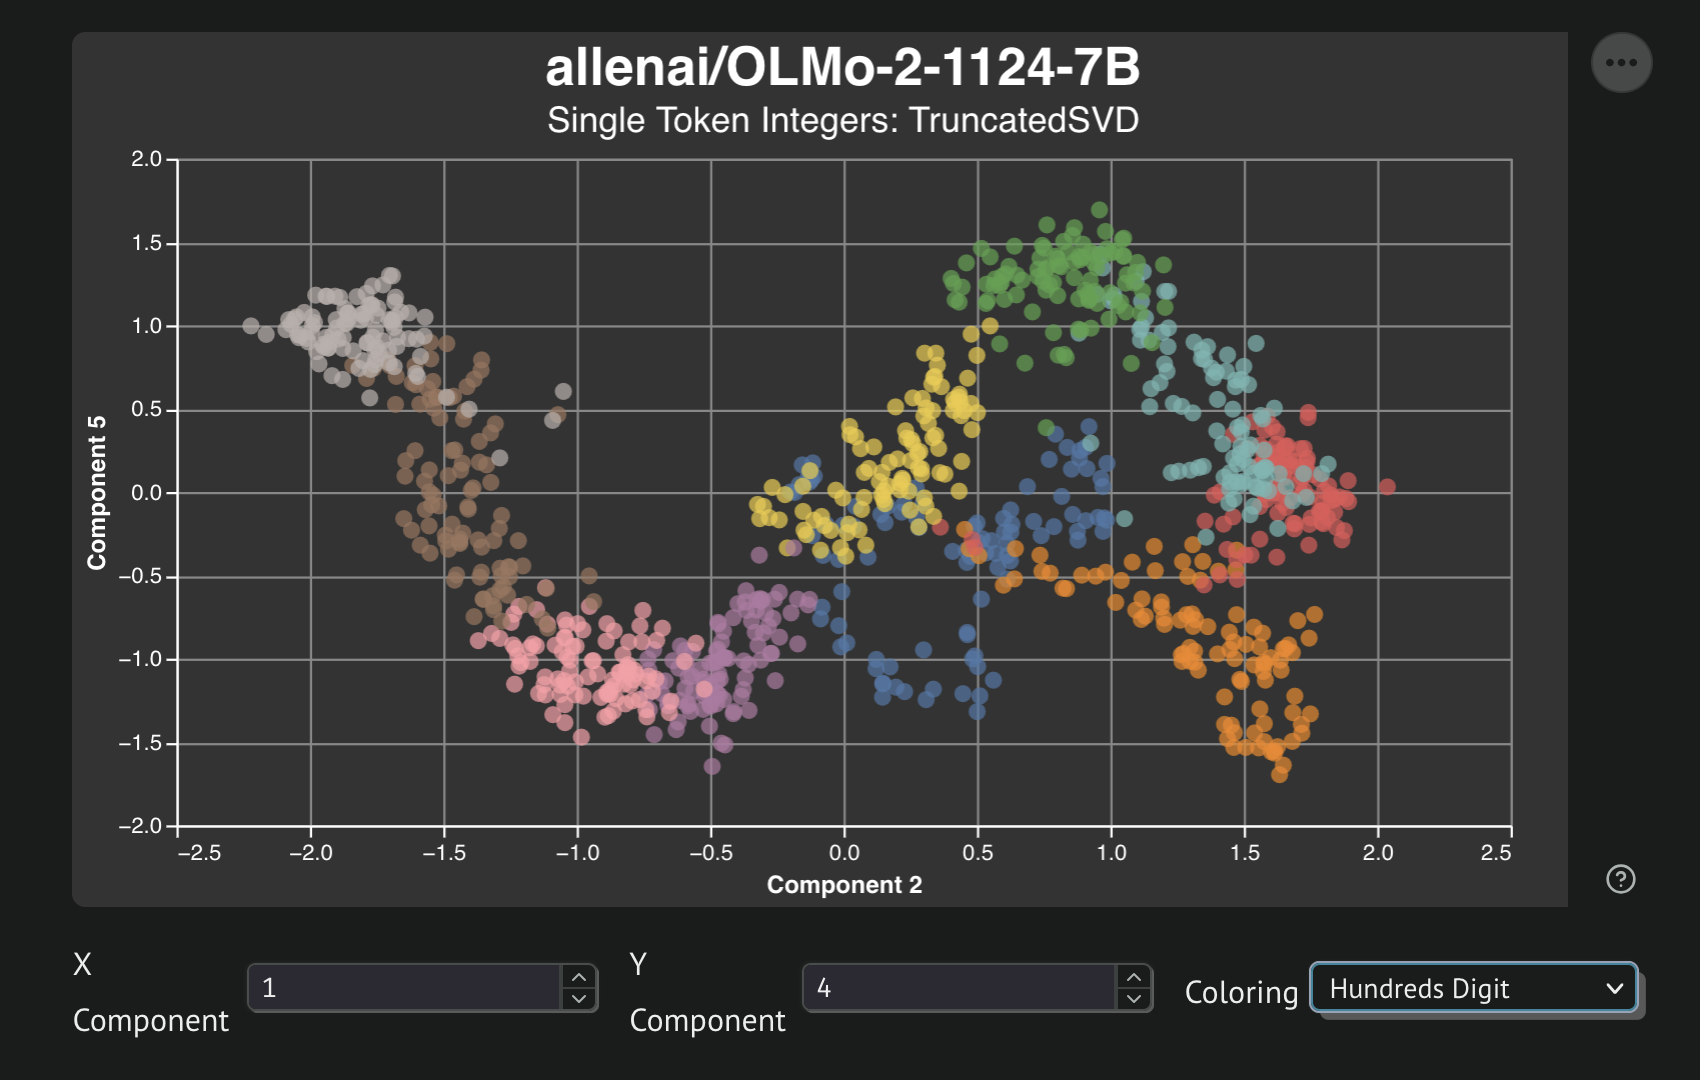
\includegraphics[keepaspectratio]{res/marimo_dashboard.png}}
\caption{Plotting component for the Marimo dashboard.}
\end{figure}

\chapter{Embeddings Analysis}\label{embeddings-analysis}

The analytic part of this work consists in the search for structures in
LLM numerical embeddings.

As stated previously, recent open source models mostly employ an L2R
tokenization scheme. There are no large scale open source models using
R2L tokenization as of the time of writing, but the improvement in
performance observed when using R2L tokenization in L2R-trained models
could be a hint that L2R embedding representations still have similar
properties to the R2L ones.

\section{Methodology}\label{methodology}

Two models are taken in consideration:

\begin{itemize}
\item
  OLMo-2-1124-7B is a model by AllenAI, which is favorable to research
  uses thanks to the full disclosure of training data, code, logs and
  checkpoints
\item
  Llama-3.2-1B-Instruct, due to being a small and manageable model to do
  analysis with on limited hardware
\end{itemize}

For each of these, dimensionality reduction is applied through PCA, SVD,
t-SNE and UMAP, and the results are used to produce 2D and 3D
visualization meant to show the geometric structure that the
representation assume in the space.

\section{OLMo-2-1124-7B}\label{olmo-2-1124-7b}

\subsection{Linear analysis}\label{linear-analysis}

\begin{figure}
\centering
\pandocbounded{\includesvg[keepaspectratio]{plots/OLMo-2-1124-7B_00_pca_components_gradient_v1.svg}}
\caption{Principal components 1 and 2 of the OLMo model. Random
embeddings sample for comparison.}\label{fig:olmo_pca}
\end{figure}

In fig.~\ref{fig:olmo_pca}, projecting the numerical token embeddings
onto the first two principal components reveals a U-shaped curve. This
structure constitutes a one-dimensional manifold embedded within the
two-dimensional principal component space.

The manifold structure is particularly significant because it
demonstrates that numerical tokens do not occupy the embedding space
randomly. Instead, they follow a constrained path that preserves
numerical relationships, suggesting that the model has learned to encode
ordering properties of the numbers within its representation. The
gradient is particularly smooth, suggesting that similar numbers
maintain spatial proximity in the reduced space.

\begin{figure}
\centering
\pandocbounded{\includesvg[keepaspectratio]{plots/OLMo-2-1124-7B_02_svd_components_gradient_v1.svg}}
\caption{SVD for the two main components of the OLMo model, with random
embeddings sample for comparison}\label{fig-olmo-svd}
\end{figure}

The SVD visualization, lacking the data centering done in the PCA, shows
a much more consistent geometric structure, suggesting that the encoding
of information might be done in absolute distances rather than just with
relative positioning between data points.

\begin{figure}
\centering
\pandocbounded{\includesvg[keepaspectratio]{plots/OLMo-2-1124-7B_03_svd_digit_visualizations_v1.svg}}
\caption{SVD coloring done by digit length and hundreds digit,
highlighting the clustering properties of the
embeddings.}\label{fig-olmo-svd-digits}
\end{figure}

There is also a very notable recursive, fractal structure, repeating
itself for numbers with one, two and three digits.

\subsubsection{Explained variance}\label{explained-variance}

\begin{figure}
\centering
\pandocbounded{\includesvg[keepaspectratio]{plots/OLMo-2-1124-7B_01_pca_variance_overview_v1.svg}}
\caption{OLMo PCA - explained variance
overview}\label{fig-olmo-variance}
\end{figure}

The explained variance by component plot (left) shows a sharp drop
within the first few components, meaning that the first principal
components capture dramatically more variance than subsequent ones. The
cumulative explained variance shows that approximatively 600 principal
components are needed to reach 90\% of explained variance.

By this we can conclude that the embeddings have a much lower intrinsic
dimensionality than their full 4096 dimensions, and that they lie on a
low-dimensional manifold in the full representation space. Only
one-fifth of the total embedding space is necessary to capture 90\% of
the variance.

\subsection{Non-linear analysis}\label{non-linear-analysis}

\begin{figure}
\centering
\pandocbounded{\includesvg[keepaspectratio]{plots/OLMo-2-1124-7B_07_tsne_components_gradient_v1.svg}}
\caption{t-SNE visualization for OLMo embeddings.}\label{fig-olmo-tsne}
\end{figure}

\begin{longtable}[]{@{}ll@{}}
\toprule\noalign{}
\textbf{Parameter} & \textbf{Value} \\
\midrule\noalign{}
\endhead
\bottomrule\noalign{}
\tabularnewline
\caption{t-SNE hyperparameters for the presented plots.
\{\#tbl-tsne-params\}}
\endlastfoot
perplexity & 75 \\
max\_iter & 3000 \\
learning\_rate & 50 \\
early\_exaggeration & 20 \\
random\_state & 42 \\
\end{longtable}

The t-SNE visualization shows a distinctive branching pattern emanating
from a central region, with low numbers at the center and higher ones
radiating outward. The color progression follows these branches,
indicating that numerical sequences are preserved along each arm. The
gradient seems also to transition circularly; branches with gradually
increasing numbers turn around the center before abruptly getting back
to the start. When interpreting the colors as indicators of depth, it
can look like a spiral from a top-down perspective.

\begin{figure}
\centering
\pandocbounded{\includesvg[keepaspectratio]{plots/OLMo-2-1124-7B_09_umap_cosine_components_gradient_v1.svg}}
\caption{UMAP visualization with cosine
distance}\label{fig-olmo-umap-cosine}
\end{figure}

\begin{figure}
\centering
\pandocbounded{\includesvg[keepaspectratio]{plots/OLMo-2-1124-7B_11_umap_euclidean_components_gradient_v1.svg}}
\caption{UMAP visualization with Euclidean
distance}\label{fig-olmo-umap-euclidean}
\end{figure}

UMAP has been run using both Euclidean and cosine distances, since the
SVD visualization has shown that absolute distances can matter in this
model. In the UMAP case we can observe a loss of shape similar to what
happened in the PCA and SVD case. While the structure is congruent when
using Euclidean distances, segregated clusters form when representing
cosine similarity, with their predominant criterion of division being
the hundreds' digit. Using Euclidean distances gives a picture similar
to t-SNE, but projected and stretched and with more dispersion for
numbers close to zero. The spiral-like conformation is also notable
here.

\subsection{Correlation with mathematical
properties}\label{correlation-with-mathematical-properties}

By taking all the components and their correlations with the properties
we're testing for, we're able to find the most correlative
component-property pairs. Most of the components that exhibit a strong
correlation does so in terms of their magnitude (measured as the
correlation with the \(log_{10}\) of the number considered).

\begin{longtable}[]{@{}rlrr@{}}
\toprule\noalign{}
\textbf{Dimension} & \textbf{Property} & \textbf{Correlation} &
\textbf{P-Value} \\
\midrule\noalign{}
\endhead
\bottomrule\noalign{}
\tabularnewline
\caption{Feature-sequence correlations in OLMo-2.
\{\#tbl-olmo-correlations\}}
\endlastfoot
514 & magnitude & -0.673 & 8.45e-133 \\
3085 & magnitude & -0.607 & 1.65e-101 \\
2538 & magnitude & -0.567 & 3.02e-86 \\
665 & magnitude & -0.500 & 1.89e-64 \\
514 & digit\_count & -0.485 & 5.30e-60 \\
1012 & magnitude & -0.475 & 1.65e-57 \\
1012 & digit\_count & -0.463 & 3.35e-54 \\
2538 & digit\_count & -0.454 & 4.12e-52 \\
3085 & digit\_count & -0.452 & 1.77e-51 \\
3879 & magnitude & 0.447 & 3.06e-50 \\
110 & magnitude & 0.445 & 8.36e-50 \\
1820 & magnitude & 0.431 & 1.99e-46 \\
1107 & magnitude & -0.428 & 8.06e-46 \\
3502 & magnitude & 0.426 & 2.46e-45 \\
421 & magnitude & -0.424 & 7.87e-45 \\
90 & magnitude & 0.420 & 6.49e-44 \\
3548 & magnitude & 0.411 & 3.99e-42 \\
1554 & magnitude & -0.410 & 8.08e-42 \\
3085 & fibonacci\_proximity & 0.410 & 8.57e-42 \\
\end{longtable}

Magnitude and digit count would be expected to be widely encoded, and
they seem in fact the dominant factor (also, they would be correlated
with each other). The most interesting property shown here is definitely
Fibonacci\_proximity, representing the distance between the number and
the closest Fibonacci number. Having a correlation index of 0.409 with a
very small p-value would be a strong indicator that this is an important
factor in the encoding of the embeddings. However, after further
consideration it was noticed that can be explained by the strong
correlation between the Fibonacci proximity and magnitude itself
(\(\approx 0.547\), p-value \(< 1e-79\)). This confounding factor might
make the correlation by itself inconclusive, and further research would
be needed to establish the connection between the two quantities. There
are also two strong correlation with both the is\_fibonacci and the
is\_prime property, which shows the embeddings are likely encoding some
information about the primality of the number considered and their
relationship to the Fibonacci series.

\begin{figure}
\centering
\pandocbounded{\includesvg[keepaspectratio]{plots/OLMo-2-1124-7B_13_strong_property_correlations_v1.svg}}
\caption{Mathematical properties with the number of associated strongly
correlated dimensions}\label{fig-olmo-properties}
\end{figure}

\section{Llama-3.2-1B-Instruct}\label{llama-3.2-1b-instruct}

\subsection{Linear analysis}\label{linear-analysis-1}

\begin{figure}
\centering
\pandocbounded{\includesvg[keepaspectratio]{plots/Llama-3.2-1B-Instruct_00_pca_components_gradient_v1.svg}}
\caption{PCA visualization of Llama embeddings.}\label{fig-llama-pca}
\end{figure}

The PCA projection shows a continuous, arc-shaped curved manifold, with
smoother transitions between numbers and a distinct separation with
numbers close to 0. As with what was seen with OLMo, it looks like the
PCA centering might end up destroying geometric relationships that are
better preserved in the SVD visualizations.

\begin{figure}
\centering
\pandocbounded{\includesvg[keepaspectratio]{plots/Llama-3.2-1B-Instruct_02_svd_components_gradient_v1.svg}}
\caption{SVD visualization of Llama embeddings}\label{fig-llama-svd}
\end{figure}

The SVD plot shows a remarkably linear arrangement - numbers form an
almost straight diagonal line from small (yellow) to large (purple)
values. This linear structure is much more pronounced than OLMo-2's
curved SVD patterns, and it is a unique shape rather than a recursive,
recurring pattern.

\begin{figure}
\centering
\pandocbounded{\includesvg[keepaspectratio]{plots/Llama-3.2-1B-Instruct_03_svd_digit_visualizations_v1.svg}}
\caption{Llama SVD visualization by digit}\label{fig-llama-svd-digits}
\end{figure}

The digit-based coloring reveals clear but subtle clustering by
mathematical properties. Unlike OLMo-2's distinct spatial territories,
Llama-3.2 shows gradual transitions along the linear arrangement while
maintaining digit-based organization patterns.

\subsubsection{Explained variance}\label{explained-variance-1}

\begin{figure}
\centering
\pandocbounded{\includesvg[keepaspectratio]{plots/Llama-3.2-1B-Instruct_01_pca_variance_overview_v1.svg}}
\caption{Llama PCA explained variance.}\label{fig-llama-variance}
\end{figure}

The explained variance plot reveals slightly higher information
concentration than OLMo-2. Llama-3.2 reaches 90\% explained variance
with approximately 500 components compared to OLMo-2's 500 components.
This suggests more efficient numerical encoding in the smaller model.

\subsection{Non-Linear analysis}\label{non-linear-analysis-1}

These nonlinear projections reveal dramatically different organizational
patterns from both the linear methods and from OLMo-2's structures.

\begin{figure}
\centering
\pandocbounded{\includesvg[keepaspectratio]{plots/Llama-3.2-1B-Instruct_07_tsne_components_gradient_v1.svg}}
\caption{t-SNE structure in Llama}\label{fig-llama-tsne}
\end{figure}

The t-SNE visualization is very unusual, and show continuous, winding
structures that might look like they had been uncoiled or unwound from a
higher-dimensional spiral arrangement. The mathematical progression
follows these winding paths smoothly. This can be informative, as for
their particularly keen encoding of the Fibonacci sequence, as will be
shown successively.

\begin{figure}
\centering
\pandocbounded{\includesvg[keepaspectratio]{plots/Llama-3.2-1B-Instruct_09_umap_cosine_components_gradient_v1.svg}}
\caption{UMAP with cosine similarity in
Llama}\label{fig-llama-umap-cosine}
\end{figure}

\begin{figure}
\centering
\pandocbounded{\includesvg[keepaspectratio]{plots/Llama-3.2-1B-Instruct_10_umap_cosine_digit_visualizations_v1.svg}}
\caption{Clustering in UMAP with cosine
similarity}\label{fig-llama-umap-cosine-digits}
\end{figure}

\begin{figure}
\centering
\pandocbounded{\includesvg[keepaspectratio]{plots/Llama-3.2-1B-Instruct_11_umap_euclidean_components_gradient_v1.svg}}
\caption{UMAP with Euclidean distance in
Llama}\label{fig-llama-umap-euclidean}
\end{figure}

The UMAP visualization is resembling the OLMo's one. It's also
interesting to see that changing the distance function to Euclidean
doesn't have particular effects, unlike the previous OLMo visualization.

\subsection{Correlation with mathematical
properties}\label{correlation-with-mathematical-properties-1}

\begin{figure}
\centering
\pandocbounded{\includesvg[keepaspectratio]{plots/Llama-3.2-1B-Instruct_13_strong_property_correlations_v1.svg}}
\caption{Dimensions strongly correlated with properties in Llama
3.2}\label{fig-llama-properties}
\end{figure}

In this case we see a lot more components directly encoding for
digit\_count, as well as for parity. There are 12 strongly correlated
components with primality and 10 with being a Fibonacci number. There is
still a big number of components strongly correlated with the
fibonacci\_proximity, which would need further analysis to fully
establish whether their sensitivity to magnitude dominates over the
detection of Fibonacci numbers.

\chapter{Conclusions}\label{conclusions}

This thesis investigated whether Large Language Models develop
structured numerical representations that might share organizational
principles with the specialized representations observed in mathematical
savants. Through analysis of numerical embeddings in OLMo-2-1124-7B and
Llama-3.2-1B-Instruct, we found evidence of systematic mathematical
structure within learned representations.

\section{Key Findings}\label{key-findings}

\subsection{Structured Numerical
Embeddings}\label{structured-numerical-embeddings}

Our analysis revealed that numerical tokens are not randomly distributed
in embedding space but follow organized patterns:

\textbf{Geometric Organization}: Principal component analysis showed
that numerical embeddings lie on low-dimensional manifolds. OLMo-2
exhibited U-shaped curves with recursive patterns across digit ranges,
while Llama-3.2 displayed more linear arrangements. Both models required
only \textasciitilde500 components to capture 90\% of variance,
indicating substantial dimensionality reduction from the full
4096-dimensional space.

\textbf{Mathematical Property Correlations}: Multiple embedding
dimensions showed *significant correlations with mathematical
properties:

\begin{itemize}
\tightlist
\item
  Magnitude and digit count exhibited the strongest correlations (r
  \textgreater{} 0.67) - Primality was encoded across multiple
  dimensions - Fibonacci number proximity showed notable correlations,
  though potentially influenced by magnitude effects
\item
  Binary properties like evenness were systematically represented
\end{itemize}

The consistent organization of numerical embeddings according to
mathematical properties suggests that neural language models might
spontaneously develop structured representations during training. This
organization goes beyond simple ordering, incorporating complex
mathematical relationships like primality and sequence membership.

\section{Limitations}\label{limitations}

The analysis was limited to two models and a specific set of
mathematical properties. The relationship between Fibonacci proximity
and magnitude highlights the challenge of isolating specific property
detectors from general ordering mechanisms. Further investigation with
controlled experiments would be needed to establish causal
relationships.

Whether these findings extend to larger models, different architectures,
or other mathematical domains remains to be determined. The observed
structures may reflect training data properties as much as emergent
organizational principles.

\section{Future Directions}\label{future-directions}

This work suggests several research directions: investigating
mathematical representations across model scales and architectures,
exploring computed embedding approaches that leverage discovered
geometric structures, and examining whether similar organizational
principles apply to other domains where specialized representations
might be beneficial.

The findings contribute to understanding how neural language models
organize mathematical information and suggest that structured
representations may emerge naturally in systems trained on numerical
data. While modest in scope, these results provide a foundation for
further investigation into the relationship between representational
structure and mathematical reasoning capabilities in artificial systems.

\chapter*{Bibliography}\label{bibliography}
\addcontentsline{toc}{chapter}{Bibliography}

\phantomsection\label{refs}
\begin{CSLReferences}{1}{0}
\bibitem[\citeproctext]{ref-ali2024}
Ali, M., Fromm, M., Thellmann, K., Rutmann, R., Lübbering, M., Leveling,
J., Klug, K., Ebert, J., Doll, N., Buschhoff, J. S., Jain, C., Weber, A.
A., Jurkschat, L., Abdelwahab, H., John, C., Suarez, P. O., Ostendorff,
M., Weinbach, S., Sifa, R., \ldots{} Flores-Herr, N. (2024, March 17).
\emph{Tokenizer {Choice For LLM Training}: {Negligible} or {Crucial}?}
\url{https://doi.org/10.48550/arXiv.2310.08754}

\bibitem[\citeproctext]{ref-golkar2023}
Golkar, S., Pettee, M., Eickenberg, M., Bietti, A., Cranmer, M.,
Krawezik, G., Lanusse, F., McCabe, M., Ohana, R., Parker, L., Blancard,
B. R.-S., Tesileanu, T., Cho, K., \& Ho, S. (2023, October 4).
\emph{{xVal}: {A Continuous Number Encoding} for {Large Language
Models}}. \url{https://doi.org/10.48550/arXiv.2310.02989}

\bibitem[\citeproctext]{ref-huh2024}
Huh, M., Cheung, B., Wang, T., \& Isola, P. (2024, May 13). \emph{The
{Platonic Representation Hypothesis}}.
\url{https://doi.org/10.48550/arXiv.2405.07987}

\bibitem[\citeproctext]{ref-islam2022}
Islam, M. M., Aguilar, G., Ponnusamy, P., Mathialagan, C. S., Ma, C., \&
Guo, C. (2022, April 22). \emph{A {Vocabulary-Free Multilingual Neural
Tokenizer} for {End-to-End Task Learning}}.
\url{https://doi.org/10.48550/arXiv.2204.10815}

\bibitem[\citeproctext]{ref-kantamneni2025}
Kantamneni, S., \& Tegmark, M. (2025, February 2). \emph{Language
{Models Use Trigonometry} to {Do Addition}}.
\url{https://doi.org/10.48550/arXiv.2502.00873}

\bibitem[\citeproctext]{ref-bitter-lesson-tokenization}
lucalp. (2025, June 24). \emph{The {Bitter Lesson} is coming for
{Tokenization} \textbar{} ⛰️ lucalp}.
\url{https://lucalp.dev/bitter-lesson-tokenization-and-blt/}

\bibitem[\citeproctext]{ref-mcinnes2020}
McInnes, L., Healy, J., \& Melville, J. (2020, September 18).
\emph{{UMAP}: {Uniform Manifold Approximation} and {Projection} for
{Dimension Reduction}}. \url{https://doi.org/10.48550/arXiv.1802.03426}

\bibitem[\citeproctext]{ref-mcleish2024}
McLeish, S., Bansal, A., Stein, A., Jain, N., Kirchenbauer, J.,
Bartoldson, B. R., Kailkhura, B., Bhatele, A., Geiping, J.,
Schwarzschild, A., \& Goldstein, T. (2024, December 23).
\emph{Transformers {Can Do Arithmetic} with the {Right Embeddings}}.
\url{https://doi.org/10.48550/arXiv.2405.17399}

\bibitem[\citeproctext]{ref-millidge2023}
Millidge, B. (2023, February 4). \emph{Integer tokenization is insane}.
\url{http://www.beren.io/2023-02-04-Integer-tokenization-is-insane/}

\bibitem[\citeproctext]{ref-millidge2024}
Millidge, B. (2024, July 7). \emph{Right to {Left} ({R2L}) {Integer
Tokenization}}.
\url{http://www.beren.io/2024-07-07-Right-to-Left-Integer-Tokenization/}

\bibitem[\citeproctext]{ref-murray2010}
Murray, A. L. (2010). Can the existence of highly accessible concrete
representations explain savant skills? {Some} insights from
synaesthesia. \emph{Medical Hypotheses}, \emph{74}(6), 1006--1012.
\url{https://doi.org/10.1016/j.mehy.2010.01.014}

\bibitem[\citeproctext]{ref-pagnoni2024}
Pagnoni, A., Pasunuru, R., Rodriguez, P., Nguyen, J., Muller, B., Li,
M., Zhou, C., Yu, L., Weston, J., Zettlemoyer, L., Ghosh, G., Lewis, M.,
Holtzman, A., \& Iyer, S. (2024, December 13). \emph{Byte {Latent
Transformer}: {Patches Scale Better Than Tokens}}.
\url{https://doi.org/10.48550/arXiv.2412.09871}

\bibitem[\citeproctext]{ref-radford2019}
Radford, A., Wu, J., Child, R., Luan, D., Amodei, D., \& Sutskever, I.
(2019). \emph{Language {Models} are {Unsupervised Multitask Learners}}.
\url{https://www.semanticscholar.org/paper/Language-Models-are-Unsupervised-Multitask-Learners-Radford-Wu/9405cc0d6169988371b2755e573cc28650d14dfe}

\bibitem[\citeproctext]{ref-singh2024}
Singh, A. K., \& Strouse, D. J. (2024, February 22). \emph{Tokenization
counts: The impact of tokenization on arithmetic in frontier {LLMs}}.
\url{https://doi.org/10.48550/arXiv.2402.14903}

\bibitem[\citeproctext]{ref-skalse2023}
Skalse, J. (2023). \emph{Some {Arguments Against Strong Scaling}}.
\url{https://www.lesswrong.com/posts/DvCLEkr9pXLnWikB8/some-arguments-against-strong-scaling}

\bibitem[\citeproctext]{ref-bitter-lesson}
Sutton, R. (2019, March 13). \emph{The {Bitter Lesson}}.
\url{http://www.incompleteideas.net/IncIdeas/BitterLesson.html}

\bibitem[\citeproctext]{ref-vaswani2023}
Vaswani, A., Shazeer, N., Parmar, N., Uszkoreit, J., Jones, L., Gomez,
A. N., Kaiser, L., \& Polosukhin, I. (2023, August 1). \emph{Attention
{Is All You Need}}. \url{http://arxiv.org/abs/1706.03762}

\end{CSLReferences}

\backmatter
\end{document}
